\documentclass[ ../main.tex]{subfiles}
\providecommand{\mainx}{..}
\begin{document}
\section{Perfect hash filter: a practical implementation of the random positive approximate set model}
\label{sec:phf}
\begin{notation}
The \emph{bit set} $\{0,1\}$ is denoted by $\BitSet$. The set of all bit strings of length $n$ is the Cartesian product $\BitSet^n$ where $\Card{\BitSet^n} = 2^n$. The \emph{empty string} is denoted by $\epsilon$ where $\BitSet^0 = \{\epsilon\}$. The set of all bit strings of length $0$ to $n$ is denoted by $\BitSet^{\leq n} = \bigcup_{j=0}^{n} \BitSet^j$ where $\Card{\BitSet^{\leq n}} = 2^{n+1} - 1$. The countably infinite set of all bit strings (of any length) is denoted by $\BitSet^{*} = \lim_{n \to \infty} \BitSet^{\leq n}$.
\end{notation}

The \emph{Bloom filter}\cite{bf} is a well-known data structure that implements a \emph{random positive approximate set} over $\BitSet^{*}$ and obtains a space complexity given approximately by
\begin{equation}
    -1.44 \log_2 \fprate \; \si{bits \per element}\,.
\end{equation}
We consider an alternative data structure, denoted the \gls{gls-phf} that also implements the \emph{random positive approximate set} over $\BitSet^*$ and compares favorably to the Bloom filter in some ways.

A hash function is related to countable sets $\BitSet^*$ and $\BitSet^n$ and is given by the following definition.
\begin{definition}
A \emph{hash function} $\hash \colon \BitSet^* \mapsto \BitSet^n$ is a function such that all bit strings of arbitrary-length are mapped (hashed) to bit strings of fixed-length $n$.
\end{definition}
For a given $x \in \BitSet^*$, $y = \hash(x) \in \BitSet^*_n$ is denoted the \emph{hash} of $x$. The \gls{gls-phf} depends on a \gls{gls-ph} as given by the following definition.
\begin{definition}
A perfect hash function of the set $\Set{S}$, denoted by
\begin{equation}
    \ph_{\Set{S}} \colon \BitSet^* \mapsto \mathbb{Z}^{+}\,,
\end{equation}
is a hash function such that the mapping from $\Set{S}$ to $\mathbb{Z}^+$ is \emph{one-to-one}.
\end{definition}
The \emph{load factor} of $\ph_{\Set{S}}$ is given by the following definition.
\begin{definition}
\label{def:loadfactor}
The load factor of $\ph_{\Set{S}}$ is a rational number given by
\begin{equation}
\label{eq:loadfactor}
    r = \frac{m}{N}\,,
\end{equation}
where $m = \Card{\Set{S}}$, $N \geq m$, and $N$ is the maximum hash of $\ph_{\Set{S}}$.
\end{definition}
\begin{definition}
A \emph{minimal} perfect hash function has a load factor $1$, i.e., the mapping from $\Set{S}$ to $\mathbb{Z}^+$ is \emph{one-to-one} and \emph{onto}.
\end{definition}

The \gls{gls-phf} is a data structure given by the following definition.
\begin{definition}
The \gls{gls-phf} is a data structure that implements\footnote{In \cref{thm:fp_rate}, we prove the \gls{gls-phf} implements the static approximate set.} the abstract data type of the \emph{positive approximate set} where the universe of elements is given by $\BitSet^*$.
\end{definition}


The \emph{Perfect Hash Filter} is a product type $\textrm{PerfectHashFilter} = \textrm{BitMatrix} \times \textrm{PerfectHash}$ and a set of functions
\begin{enumerate}
\item $\Contains \colon \BitSet^* \times \textrm{PerfectHashFilter}]$
\end{enumerate}



tuple of type $[\textrm{BitMatrix}]$ that implements\footnote{In \cref{thm:fp_rate}, we prove the \gls{gls-phf} implements the static approximate set.} the abstract data type of the \emph{positive approximate set} where the universe of elements is given by $\BitSet^*$.


The \emph{minimal} perfect hash filter given by the following definition.
\begin{definition}
The \emph{minimal} perfect hash filter is a perfect hash filter with a load factor $1$, i.e., every element $x$ in the set being approximated is \emph{perfectly hashed}.
\end{definition}
Replacing the \emph{perfect hash function} with a \emph{$k$-perfect hash function}, where disjoint subsets of up to $k$ elements may collide, generalizes the \gls{gls-phf} into an approximate set where both \emph{false positives} and \emph{false negatives} are possible.\footnote{We may also simply approximate a subset of a set $\Set{S}$ to support non-zero false negative rates, but \emph{$k$-perfect hashing} generates a more efficient solution.}

\Cref{alg:PHF,alg:PHF_has} describe the implementations of \MakeApproxSet and \Contains respectively.
\begin{algorithm}[h]
    \caption{Implementation of \protect\MakeApproxSet}
    \label{alg:PHF}
    \SetKwProg{func}{function}{}{}
    \KwIn
    {
        \begin{itemize}
            \item[$\Set{S}$] The \gls{gls-finiteset} to approximate.
            \item[$\fprate$] The \gls{gls-fprate}.
            \item[$r$] The \gls{gls-loadfactor}.
        \end{itemize}
    }
    \KwOut
    {
        A \gls{gls-phf} that approximates $\Set{S}$ with a \gls{gls-fprate} $\fprate$ and a \gls{gls-loadfactor} $r$.
    }
    \func{\MakeApproxSet{$\Set{S}, \fprate \given r$}}
    {
        $\ph_{\Set{S}} \gets$ \PHFgen{$\Set{S}$, $r$}\;
        $N \gets \left\lceil \Card{\Set{S}} / r \right\rceil$\;
        $M \gets \left\lceil -\log_2\!\left(\fprate\right) \right\rceil$\;
        $\matrx{V} \gets N$-by-$M$ bit matrix\;
        \For{$x \in \Set{S}$}
        {
            $i \gets \ph_{\Set{S}}\!\left(x\right)$\;
            $h \gets$ \ro{$x$}$\mod M$\;
            $\matrx{V}\!\left[i\right] \gets h$\;
        }
        \tcp{This tuple is sufficient to code the \gls{gls-phf}.}
        \Return $\left(\matrx{V}, \ph_{\Set{S}}\right)$\;
    }
\end{algorithm}
\begin{algorithm}[h]
    \caption{Implementation of \protect\Contains}
    \label{alg:PHF_has}
    \SetKwProg{func}{function}{}{}
    \KwIn
    {
        \begin{enumerate}
            \item[$\PASet{S}$] The \gls{gls-phf} data structure that approximates $\Set{S}$ with a false positive rate $\fprate$ and a load factor $r$.
            \item[$x$] The bit string to test membership of in $\PASet{S}$.
        \end{enumerate}
    }
    \KwOut
    {
        $\True$ if $x \in \Set{S}$, otherwise $\True$ with probability $\fprate$ and false with probability $1 - \fprate$.
    }
    \func{\Contains{$\PASet{S}, x$}}
    {
        $M \gets \Columns(\matrx{V})$\;
        $N \gets \Rows(\matrx{V})$\;
        $i \gets \ph_{\Set{S}}\!\left(x\right)$\;
        $h \gets \hash(x) \mod N$\;
        \Return{$\matrx{V}\!\left[i\right] = h$}\;
    }
\end{algorithm}

\begin{example}
Consider a set $\Set{S} = \{x_1, x_2, x_3\}$ and suppose we wish to approximate this set with a false positive rate $\fprate = 2^{-3}$. The perfect hash filter depicted by \cref{fig:PHFilter} is a representation of this \emph{frozen approximate set}.
\end{example}
\begin{figure}
\caption[Perfect hash filter]{A perfect hash filter implementing a static approximate set $\{x_1,x_2,x_3\}$ with a false positive rate $\fprate = 2^{-3}$ and a load factor $r = \frac{3}{5}$.}
\label{fig:PHFilter}
\centering
%% Creator: Inkscape inkscape 0.92.1, www.inkscape.org
%% PDF/EPS/PS + LaTeX output extension by Johan Engelen, 2010
%% Accompanies image file 'phfilter.pdf' (pdf, eps, ps)
%%
%% To include the image in your LaTeX document, write
%%   \input{<filename>.pdf_tex}
%%  instead of
%%   \includegraphics{<filename>.pdf}
%% To scale the image, write
%%   \def\svgwidth{<desired width>}
%%   \input{<filename>.pdf_tex}
%%  instead of
%%   \includegraphics[width=<desired width>]{<filename>.pdf}
%%
%% Images with a different path to the parent latex file can
%% be accessed with the `import' package (which may need to be
%% installed) using
%%   \usepackage{import}
%% in the preamble, and then including the image with
%%   \import{<path to file>}{<filename>.pdf_tex}
%% Alternatively, one can specify
%%   \graphicspath{{<path to file>/}}
%% 
%% For more information, please see info/svg-inkscape on CTAN:
%%   http://tug.ctan.org/tex-archive/info/svg-inkscape
%%
\begingroup%
  \makeatletter%
  \providecommand\color[2][]{%
    \errmessage{(Inkscape) Color is used for the text in Inkscape, but the package 'color.sty' is not loaded}%
    \renewcommand\color[2][]{}%
  }%
  \providecommand\transparent[1]{%
    \errmessage{(Inkscape) Transparency is used (non-zero) for the text in Inkscape, but the package 'transparent.sty' is not loaded}%
    \renewcommand\transparent[1]{}%
  }%
  \providecommand\rotatebox[2]{#2}%
  \ifx\svgwidth\undefined%
    \setlength{\unitlength}{261.09346686bp}%
    \ifx\svgscale\undefined%
      \relax%
    \else%
      \setlength{\unitlength}{\unitlength * \real{\svgscale}}%
    \fi%
  \else%
    \setlength{\unitlength}{\svgwidth}%
  \fi%
  \global\let\svgwidth\undefined%
  \global\let\svgscale\undefined%
  \makeatother%
  \begin{picture}(1,0.54970412)%
    \put(0,0){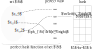
\includegraphics[width=\unitlength,page=1]{phfilter.pdf}}%
    \put(0.64566511,0.38339903){\color[rgb]{0,0,0}\makebox(0,0)[lb]{\smash{\ro{$x_3$}}}}%
    \put(0.69732565,0.38431659){\color[rgb]{0,0,0}\makebox(0,0)[lb]{\smash{}}}%
    \put(0.71703304,0.37723766){\color[rgb]{0,0,0}\makebox(0,0)[lb]{\smash{}}}%
    \put(0.57909529,0.43867283){\color[rgb]{0,0,0}\makebox(0,0)[lb]{\smash{$1$}}}%
    \put(0.57909529,0.3592831){\color[rgb]{0,0,0}\makebox(0,0)[lb]{\smash{$2$}}}%
    \put(0.57909529,0.27989338){\color[rgb]{0,0,0}\makebox(0,0)[lb]{\smash{$3$}}}%
    \put(0.57909529,0.20050357){\color[rgb]{0,0,0}\makebox(0,0)[lb]{\smash{$4$}}}%
    \put(0.57909529,0.12111369){\color[rgb]{0,0,0}\makebox(0,0)[lb]{\smash{$5$}}}%
    \put(0.09855085,0.52){\color[rgb]{0,0,0}\makebox(0,0)[lb]{\smash{set $\Set{S}$}}}%
    \put(0,0){\includegraphics[width=\unitlength,page=2]{phfilter.pdf}}%
    \put(0.07598078,0.28851046){\color[rgb]{0,0,0}\makebox(0,0)[lb]{\smash{$x_1$}}}%
    \put(0.1214073,0.38150573){\color[rgb]{0,0,0}\makebox(0,0)[lb]{\smash{$x_3$}}}%
    \put(0.15393678,0.20004317){\color[rgb]{0,0,0}\makebox(0,0)[lb]{\smash{$x_2$}}}%
    \put(0.49244358,0.52){\color[rgb]{0,0,0}\makebox(0,0)[lb]{\smash{perfect hash}}}%
    \put(0,0){\includegraphics[width=\unitlength,page=3]{phfilter.pdf}}%
    \put(0.29706424,0.1846711){\color[rgb]{0,0,0}\makebox(0,0)[lb]{\smash{\ph{$x_3$}}}}%
    \put(0.34872462,0.1855885){\color[rgb]{0,0,0}\makebox(0,0)[lb]{\smash{}}}%
    \put(0.1,0.00775393){\color[rgb]{0,0,0}\makebox(0,0)[lb]{\smash{perfect hash function of set $\Set{S}$}}}%
    \put(0,0){\includegraphics[width=\unitlength,page=4]{phfilter.pdf}}%
    \put(0.86775057,0.52){\color[rgb]{0,0,0}\makebox(0,0)[lb]{\smash{hash}}}%
    \put(0.74,0.00775393){\color[rgb]{0,0,0}\makebox(0,0)[lb]{\smash{$5$-by-$3$ bit matrix $\matrx{V}$}}}%
    \put(0.81794979,0.35610106){\color[rgb]{0,0,0}\makebox(0,0)[lb]{\smash{$0$}}}%
    \put(0.89180672,0.35610251){\color[rgb]{0,0,0}\makebox(0,0)[lb]{\smash{$1$}}}%
    \put(0.95581599,0.35610243){\color[rgb]{0,0,0}\makebox(0,0)[lb]{\smash{$1$}}}%
    \put(0,0){\includegraphics[width=\unitlength,page=5]{phfilter.pdf}}%
  \end{picture}%
\endgroup%

\end{figure}

We make the following set of assumptions. See \cite{oph} for more on these assumptions.
\begin{assumption}
The set $\Set{S}$ consists of $m$ elements, where each element is drawn uniformly at random without replacement from $\BitSet^*$.
\end{assumption}
\begin{assumption}
The perfect hash function $\ph_{\Set{S}}$ approximates a random oracle.
\end{assumption}
\begin{assumption}
\label{asm:ro}
The hash function $\ro \colon \BitSet^* \mapsto \BitSet^*_n$ approximates a random oracle.
\end{assumption}

The \gls{gls-phf} is an implementation of a \emph{static approximate set} as given by the following theorem.
\begin{theorem}
\label{thm:fp_rate}
A \gls{gls-phf} is an implementation of \emph{static approximate set} with a false positive rate that is a rational number given by
\begin{equation}
\label{eq:fp_rate}
    \fprate \in \left\{ 2^{-k} \colon k \in \mathbb{Z}^+\right\} \subset \left(0, 1\right]\,.
\end{equation}
\end{theorem}
\begin{proof}
For the \gls{gls-phf} to be an implementation of approximate set $\PASet{S} \supset \Set{S}$, by \cref{def:approx_set} the following conditions must be met:
\begin{enumerate}
\item\label{itm:fp_rate_1} For all $x \in \Set{S}$, $x \in \PASet{S}$ returns \True.
\item\label{itm:fp_rate_2} For any $x \notin \Set{S}$, $x \in \PASet{S}$ returns \True with probability $\fprate$ and \False with probability $1 - \fprate$.
\end{enumerate}

First, we prove condition \ref{itm:fp_rate_1}. For some $x \in \BitStringSet$,
let $i = \ph_{\Set{X}}(x)$. For \Contains{$\PASet{S}$,$x$} to return \True, row $\matrx{V}[i]$ must equal the hash given by \hash{$x$}. Since \ph$_{\Set{S}}$ perfectly hashes all $y \in \Set{S}$ and $x \in \Set{S}$, no other member of $\Set{S}$ hashes ?, and $\matrx{V}[i]$ is explicitly set to the hash $\hash(x)$ during the construction of the \gls{gls-phf} as given by \cref{alg:PHF}.

Second, we prove condition \ref{itm:fp_rate_2}. Observe that $\ph_{\Set{S}}$ is a hash function that takes any $x \in \BitSet^*$ and maps it to an integer between $1$ and $N$. The corresponding row of $\matrx{V}$ consists of $M$ bits. There are $2^M$ possible bit strings of length $M$ and, by \cref{asm:ro}, \hash uniformly distributes over these possibilities. Thus, for $x \notin \Set{S}$, the probability that \hash{$x$} is equal to the corresponding $M$ bits is given by the false positive rate
\begin{equation}
\fprate = 2^{-M}\,.
\end{equation}
Since $M$ is any non-negative integer, the false positive rate is given by \cref{eq:fp_rate}.
\end{proof}

\subsection{Space complexity}
The minimum possible bit length of a data structure implementing the abstract data type of the \emph{approximate set} is given by the following postulate.
\begin{postulate}
\label{pst:approx_l_b}
The information-theoretic lower-bound of a data structure that implements the \emph{approximate set} abstract data type has an \emph{expected} bit length given by
\begin{equation}
    -\log_2 \fprate \; \si{bits \per element}\,,
\end{equation}
where $\fprate$ is the false positive rate.
\end{postulate}

The \emph{expected} bit length of the \emph{minimal} \gls{gls-phf} has a lower-bound given by the following theorem.
\begin{theorem}
\label{thm:mPHF_size}
The \emph{expected} bit length of the \gls{gls-phf} with a load factor $r$ has a lower-bound given by
\begin{equation}
\label{eq:mPHF_size}
    \log_2 e - \frac{1}{r} \log_2 \fprate - \left(\frac{1}{r} - 1\right) \log_2\left(\frac{1}{1-r}\right)\; \si{bits \per element}\,,
\end{equation}
where $\fprate$ is the false positive rate and $r$ is the load factor.
\end{theorem}
\begin{proof}
The proof comes in two parts. First, according to Theorem~3 in \cite{oph}, the \emph{expected} lower-bound for a perfect hash function with a load factor $r$ is given by
\begin{equation}
    \log_2 \mathrm{e} - \left(\frac{1}{r} - 1\right) \log_2\!\left(\frac{1}{1-r}\right) \si{bits \per element}\,.
\end{equation}
Second, a perfect hash function with a load factor $r$ maps each $x \in \Set{S}$ to a unique integer between $1$ and $\frac{m}{r}$, where $m=\Card{\Set{S}}$, which requires a bit matrix $\matrx{V}$ with $m$ rows. Also, as shown in the proof for \cref{thm:fp_rate}, a false positive rate $\fprate$ requires $M = -\log_2 \fprate$ bits. Thus, the bit matrix $\matrx{V}$ has $m$ rows and $-\log_2 \fprate$ columns, resulting in a total of
\begin{equation}
    -\frac{m}{r} \log_2 \fprate \; \si{bits}\,.
\end{equation}
Adding both parts of the proof together results in
\begin{equation}
    -\frac{m}{r} \log_2 \fprate + m \log_2 \mathrm{e} - m \left(\frac{1}{r} - 1\right) \log_2\!\left(\frac{1}{1-r}\right) \si{bits}\,.
\end{equation}
Since we are interested in the bits per element, we divide by $m$ yielding the result
\begin{equation}
    -\frac{1}{r} \log_2 \fprate + \log_2 \mathrm{e} -  \left(\frac{1}{r} - 1\right) \log_2\!\left(\frac{1}{1-r}\right) \si{bits \per element}\,.
\end{equation}
\end{proof}

\begin{corollary}
The \emph{expected} bit length of the \emph{minimal} \gls{gls-phf} has a lower-bound given by
\begin{equation}
\label{eq:mPHF_size}
    \log_2 \frac{e}{\fprate} \; \si{bits \per element}\,,
\end{equation}
where $\fprate$ is the false positive rate.
\end{corollary}
\begin{proof}
First, $1.44 \si{bits}$ is the \emph{expected} bits per element for optimally space-efficient \emph{minimal perfect hash functions}.

Second, a \emph{minimal} perfect hash function maps each $x \in \Set{S}$ to a unique integer between $1$ and $m=\Card{\Set{S}}$ which requires a bit matrix $\matrx{V}$ with $m$ rows. Also, as shown in the proof for \cref{thm:fp_rate}, a false positive rate $\fprate$ requires $M = -\log_2 \fprate$ bits. Thus, the bit matrix $\matrx{V}$ has $m$ rows and $-\log_2 \fprate$ columns, resulting in a total of
\begin{equation}
    -m \log_2 \fprate \; \si{bits}\,.
\end{equation}
Adding both parts of the proof together results in
\begin{equation}
    -m \log_2 \fprate + 1.44 m\; \si{bits}\,.
\end{equation}
Since we are interested in the bits per element, we divide by $m$ yielding the result
\begin{equation}
    1.44 - \log_2 \fprate\; \si{bits \per element}\,.
\end{equation}
\end{proof}


\begin{figure}
\centering
\caption{Optimal load factor $r^*$ for a given false positive rates $\fprate$ for \gls{gls-phf} $X$. We compute the corresponding absolute efficiency and the relative efficiency to \gls{gls-blf} $Y$.}
\label{fig:abs_eff}
\begin{tabular}{c *{3}{S[table-auto-round,
                 table-format=-1.3]}}
{$\fprate$} & {$r^*$} & {$e^*(X)$} & {$e(X,Y)$}\\
\hline
$2^{-1}$  & 0.768039 & 0.474373 & 0.684375\\ 
$2^{-2}$  & 0.898172 & 0.606835 & 0.875478\\
$2^{-3}$  & 0.951741 & 0.686016 & 0.989713\\
$2^{-4}$  & 0.97646 & 0.739545 & 1.06694\\
$2^{-5}$  & 0.988369 & 0.778099 & 1.12256\\
$2^{-6}$  & 0.994219 & 0.807064 & 1.16435\\
$2^{-7}$  & 0.997118 & 0.829528 & 1.19676\\
$2^{-8}$  & 0.998561 & 0.847402 & 1.22254\\
$2^{-9}$  & 0.999281 & 0.861932 & 1.24351\\
$2^{-10}$ & 0.999641 & 0.87396 & 1.26086\\
$2^{-20}$ & 1 & 0.932719 & 1.34563\\
$2^{-30}$ & 1 & 0.954117 & 1.3765\\
$2^{-60}$ & 1 & 0.97652 & 1.40882\\
$2^{-120}$ & 1 & 0.98812 & 1.42556\\
\end{tabular}
\end{figure}

\begin{figure}
\caption{Relative efficiency of the Perfect Hash Filter $X$ to the Bloom filter $Y$}
\label{fig:rel_eff_bf_PHF}
\centering
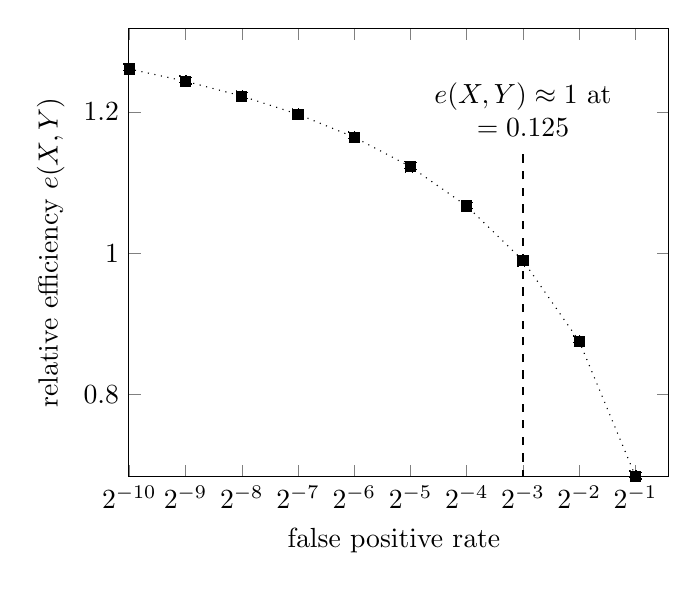
\begin{tikzpicture}
\begin{axis}[
    log basis x=2,
    xmode=log,
    ymin=.684,
    xmin=0.00097,
    xmax=.75,
    xlabel={false positive rate $\fprate$},
    ylabel={relative efficiency $e(X,Y)$},
    legend pos=north west,
    ]
    \addplot[dashed] coordinates {(0.125,0) (0.125,1.15)};
    \addplot[dotted,mark=square*] table
    {
        7.5231638e-37   1.42556
        8.6736174e-19   1.40882
        9.3132257e-10   1.3765
        9.53674316e-7   1.34563
        0.000976563     1.26086
        0.00195313      1.24351
        0.00390625      1.22254
        0.0078125       1.19676
        0.015625        1.16435
        0.03125         1.12256
        0.0625          1.06694
        0.125           0.989713
        0.25            0.875478
        0.5             0.684375
    };
    \node[label={$e(X,Y) \approx 1$ at}] at (axis cs:0.125,1.175) {};
    \node[label={$\fprate = 0.125$}] at (axis cs:0.125,1.1375) {};
  \end{axis}
\end{tikzpicture}
\end{figure}

The bit length of an object $x$ is denoted by
\begin{equation}
    \BL(x)\,,
\end{equation}
e.g., the bit length of any $x \in \BitSet^*_n$ is given by $\BL(x) = n$. The relative space efficiency metric is given by the following definition.
\begin{definition}
The relative space efficiency of a data structure $X$ to a data structure $Y$ is given by the ratio of the bit length of $Y$ to the bit length of $X$ as given by
\begin{equation}
    e(X,Y)=\frac{\BL(Y)}{\BL(X)}\,,
\end{equation}
where $\BL$ is the bit length function. There are three possibilities:
\begin{enumerate}
    \item $\RE(X,Y) < 1 \iff X$ is less efficient than $Y$.
    \item $\RE(X,Y) = 1 \iff X$ and $Y$ are equally efficient.
    \item $\RE(X,Y) > 1 \iff X$ is more efficient than $Y$.
\end{enumerate}
\end{definition}

The \emph{absolute} space efficiency of an approximate set $X$ with a false positive rate $\fprate$ is given by
\begin{equation}
    \AE\!(X) = e(X,-\log_2 \fprate)\,.
\end{equation}
An asymptotically optimal space-efficient data structure has an absolute efficiency that goes to $1$ as the cardinality $m$ of the set being approximated goes to $\infty$. The absolute efficiency of the \gls{gls-phf} is not asymptotically optimal since it has an asymptotic limit less than $1$ that is a function of the false positive rate $\fprate$ as shown in \cref{fig:abs_eff}. However, as $\fprate$ goes to $0$ the absolute efficiency goes to $1$.

\paragraph{Comparisons to the \emph{\gls{gls-blf}}.}
The \gls{gls-phf} is most suitable as an immutable data structure. It is optimized for read-many, write-once usage patterns. Once it is constructed, only on the order of
\begin{equation}
    \mathcal{O} \left( 1 \right)
\end{equation}
hash functions need to be computed to test an element for membership. The Bloom filter is suitable as a mutalbe data structure; elements may be inserted into it at any point at a cost of increasing the false positive rates. However, it requires computing on the order of
\begin{equation}
    \mathcal{O}\left(-\log \fprate\right)
\end{equation}
hash functions per membership test.

The \emph{Bloom filter} has an expected encoding size given approximately by
\begin{equation}
    -1.44 \log_2 \fprate \; \si{bits \per element}\,.
\end{equation}
The absolute efficiency of the \gls{gls-blf} is approximately $\ln 2 \approx 0.69$.

The relative efficiency of the \gls{gls-phf} to the \gls{gls-blf} is a function of the false positive rate $\fprate$ as shown in \cref{fig:rel_eff_bf_PHF,fig:abs_eff}. If $\fprate < 2^{-3}$, the \gls{gls-blf} is more space efficient; otherwise the \gls{gls-phf} is more space efficient. As $\fprate$ goes to $0$, the relative efficiency of the \gls{gls-phf} to the \gls{gls-blf} goes to $1.44$. 

\subsection{Entropy}
If the load factor is known, the cardinality of $\Set{S} \subset \PASet{S}$ is given by
\begin{equation}
    \Card{\Set{S}} = N r\,.
\end{equation}

If the load factor is not known, then the cardinality may be probabilistically estimated.
According to \cite{}, the probability mass of the perfect hash function is given by
\begin{equation}
    \RV{N} \sim \PDF{n \Given m, r}[\RV{N}] = q^{2^n-1}\left(1 - q^{2^n}\right)
\end{equation}
where
\begin{equation}
\begin{split}
	q &= 1 - \frac{(m/r)!}{(m/r)^m ((m/r)-m)!}\,,\\
	m &= \Card{\Set{S}}\,,\\
\end{split}
\end{equation}

%Since $m = N r$

It does contain some information. We know that if the bit matrix of hashes $\matrx{V}$ has $m$ rows and $k$ columns, then $\Card{\Set{S}} \leq m$ and the expected false positive rate is $\fprate=2^{-k}$.


\begin{theorem}
The random bit string that codes the \gls{gls-phf} is a \emph{maximum entropy} coder for the \emph{approximate set} abstract data type.
\end{theorem}
\begin{proof}
For a random bit $\RV{X}$ to have maximum entropy, it must be Bernoulli distribution with equiprobability, i.e.,
\begin{equation}
    \RV{X} \sim \berdist\!\left(p = \frac{1}{2}\right)\,.
\end{equation}

The \gls{gls-phf} of $\Set{S}$ is coded by two parts. The first party is a \emph{cryptographic} hash of $m$ elements in $\Set{S}$ concatenated with a bit string $b_n$, denoted by $h_k$. The \emph{cryptographic} hash function uniformly distributes over $\BitSet^{k}$, and so $h_k$ has maximum entropy.

The second part is a bit string $b_n$ of bit length $n$.
\end{proof}

The only information contained in the code, prior to memmbership test, is given by the probality mass function of the random bit length $\RV{N}$, which is a function of the cardality of the \gls{gls-finiteset} it is approximating.

The random bit length $\RV{N}$ of the string has a probability mass concentrated around
\begin{equation}
    -m \log_2 \fprate + 1.44 m\,.
\end{equation}


\begin{theorem}
An estimator of the cardinality of an approximated set represented by a \gls{gls-phf} is given by
\begin{equation}
    \hat{m} = -\frac{\BL\!\left(\PASet{S}\right)}{-\log_2 \fprate + 1.44}\,,
\end{equation}
were $\BL$ is the bit length function and $\fprate$ is the \emph{\gls{gls-fprate}}.
\end{theorem}
\begin{proof}
The \emph{expected} bit length is given by
\begin{equation*}
    \Expect{\RV{N}} = -m \log_2 \fprate + 1.44 m\,, 
    \tag{\ref{} revisited}
\end{equation*}
where $m$ is the cardinality of the approximated set. Thus, the maximumn likelihood estimator is given by assuming the bit length of the \gls{gls-phf} realizes this expectation,
\begin{equation}
    \BL(\PASet{S}) = -\hat{m} \log_2 \fprate + 1.44 \hat{m}\,.
\end{equation}
Solving for $\hat{m}$ results in the estimator
\begin{equation}
    \hat{m} = \frac{\BL(\PASet{S})}{-\log_2 \fprate + 1.44}\,.
\end{equation}
\end{proof}



\begin{theorem}
A \emph{maximum likelihood estimator} of the cardinality of an approximated set represented by a \gls{gls-phf} is given by
\begin{equation}
    \hat{m} = -\frac{\BL\!\left(\PASet{S}\right)}{-\log_2 \fprate + 1.44}\,,
\end{equation}
were $\BL$ is the bit length function and $\fprate$ is the \emph{\gls{gls-fprate}}.
\end{theorem}
\begin{proof}
The \emph{expected} bit length is given by
\begin{equation*}
    \Expect{\RV{N}} = -m \log_2 \fprate + 1.44 m\,, 
    \tag{\ref{} revisited}
\end{equation*}
where $m$ is the cardinality of the approximated set. Thus, the maximumn likelihood estimator is given by assuming the bit length of the \gls{gls-phf} realizes this expectation,
\begin{equation}
    \BL(\PASet{S}) = -\hat{m} \log_2 \fprate + 1.44 \hat{m}\,.
\end{equation}
Solving for $\hat{m}$ results in the estimator
\begin{equation}
    \hat{m} = \frac{\BL(\PASet{S})}{-\log_2 \fprate + 1.44}\,.
\end{equation}
\end{proof}
However, there is actually a simpler method. Simply count the number of rows in the matrix $\matrx{V}$.

We made trade space complexity for entropy if desired. For instance, if we find a bit string of a length around $t > -m \log_2 \fprate$ that codes the \gls{gls-phf}, then an estimate of the cardinality is given by
\begin{equation}
    \hat{\Card{\Set{S}}} = -\frac{t}{\log_2 \fprate}\,.
\end{equation}
Thus, without knowing how $t$ was chosen, we can only infer that the approximated set has a cardinality approximately between $0$ and $-\frac{t}{\log_2 \fprate}$, which has an approximate entropy of $\log_2 t$. The coding efficiency is now given by
\begin{equation}
    0 < \frac{m}{t} \leq 1\,,
\end{equation}
which is the \emph{maximum} efficiency possible for an approximate set with $\log_2 t$ entropy for the cardinality.

\subsection{C++ implementation}
\lstinputlisting
[
    float,
    language=c++,
    frame=lines,
    label={code:sas},
    caption={The C++ interface of the \emph{static approximate set}} abstract data type
]
{code/approximate_set.h}

\lstinputlisting
[
    float,
    language=c++,
    frame=lines,
    label={code:phf},
    caption={The C++ interface of the \gls{gls-phf}}
]
{code/perfect_hash_filter.h}


The theoretical \gls{gls-phf} based off of the random oracle as described by \cite{oph} is not tractable. Its purpose was to demonstrate theoretical properties.

We use a fast state-of-the-art algorithm \cite{chd} for generating perfect hash functions that requires $\alpha(r) \; \si{bits \per element}$, where $\alpha$ is a function of the \gls{gls-loadfactor} $r$ which does not obtain the \emph{expected} lower-bound. The expected bit length of this \gls{gls-phf} is given by
\begin{equation}
    -\frac{1}{r} \log_2 \fprate + \alpha(r) \; \si{bits \per element}
\end{equation}
and its absolute efficiency is given by
\begin{equation}
    \frac{-\frac{1}{r}\log_2 \fprate + \alpha(r)}{-\log_2 \fprate}
\end{equation}


The relative efficiency of the Bloom filter to the perfect hash filter is given by
\begin{equation}
     0.69 - \frac{\alpha(r)}{1.44 \log_2 \fprate}
\end{equation}
As $\fprate \to 0$, the relative efficiency goes to $0.69$. In the case of a the \emph{minimal} perfect hash filter,
\begin{equation}
    \alpha(1) = 2.07\,.
\end{equation}
The relative efficiency of the Bloom filter to the \emph{minimal} perfect hash filter is given by
\begin{equation}
    \ln 2 - \frac{1.4375}{\log_2 \fprate}\,.
\end{equation}
The point at which they are equally efficient efficient is $\fprate \approx 2^{-4}$. Thus, the \emph{minimal} perfect hash filter is more efficient if $\fprate < 2^{-4}$ and otherwise the Bloom filter is more efficient. See \cref{fig:rel_eff} for a visualization.
\begin{figure}
\caption{Relative efficiency of the Bloom filter to the \emph{minimal} perfect hash filter}
\label{fig:rel_eff}
\centering
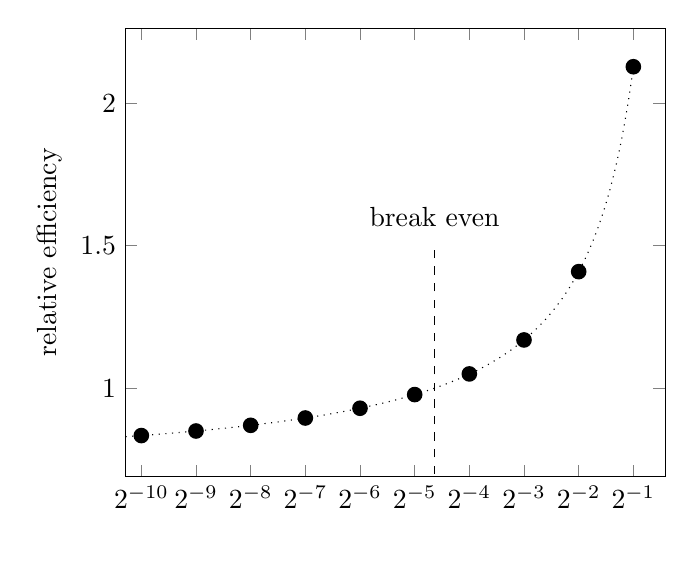
\begin{tikzpicture}
\begin{axis}[
    log basis x=2,
    xmode=log,
    ymin=.69,
    xmin=0.0008,
    xmax=.75,
    xlabel={$\fprate$},
    ylabel={relative efficiency}
    ]
    \addplot[dotted,samples=1000,domain=0.0008:.5]{-1.4375/log2(x)+.69};
    \addplot[dashed] coordinates {(0.0401879,0) (0.0401879,1.5)};
    \node[label={break even}] at (axis cs:0.0401879,1.5) {};
    \node[circle,fill,inner sep=2pt] at (axis cs:0.000976563,0.83375) {};
    \node[circle,fill,inner sep=2pt] at (axis cs:0.00195313,0.849722) {};
    \node[circle,fill,inner sep=2pt] at (axis cs:0.00390625,0.869687) {};
    \node[circle,fill,inner sep=2pt] at (axis cs:0.0078125,0.895357) {};
    \node[circle,fill,inner sep=2pt] at (axis cs:0.015625,0.929583) {};
    \node[circle,fill,inner sep=2pt] at (axis cs:0.03125,0.9775) {};
    \node[circle,fill,inner sep=2pt] at (axis cs:0.0625,1.05) {};
    \node[circle,fill,inner sep=2pt] at (axis cs:0.125,1.16917) {};
    \node[circle,fill,inner sep=2pt] at (axis cs:0.25,1.40875) {};
    \node[circle,fill,inner sep=2pt] at (axis cs:0.5,2.1275) {};
  \end{axis}
\end{tikzpicture}
\end{figure}
\end{document}